\begin{figure}[!ht]
	\centering
	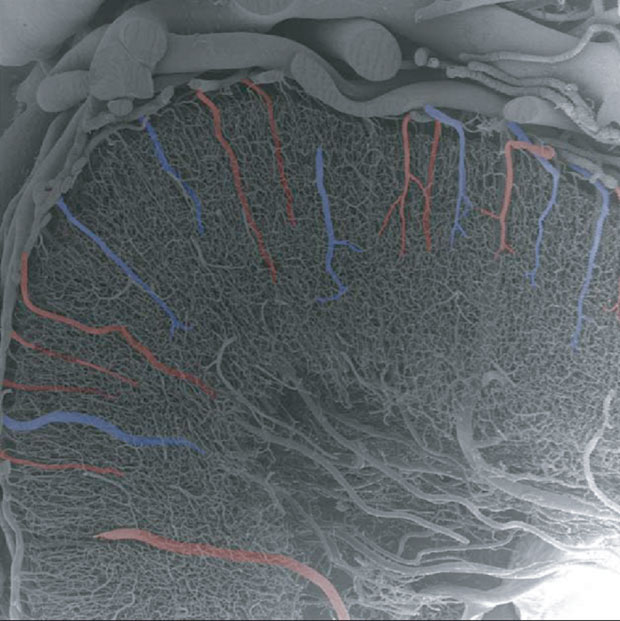
\includegraphics[width=0.9\textwidth, clip=true]{./Chapters/01_Introduction/Images/Microvasculature}
	\caption{The microvasculature of the visual cortex of a macaque. The cortex is rich in little venules that supply the cortex from blood. They are supplied with oxygen by arteries (red) and drained by cortical veins (blue). The deoxyhemoglobin accumulates by the large draining veins directly on top of the cortex. Picture adapted from Weber et al. \cite{Weber2008}.}
	\label{fig:microvasulature}
\end{figure}